\documentclass[11pt]{article}
\usepackage[margin=1in]{geometry}
\usepackage{amsmath,amssymb,booktabs,array,graphicx,hyperref,microtype}
\hypersetup{colorlinks=true,linkcolor=blue!50!black,urlcolor=blue!50!black,citecolor=black}
\usepackage{xcolor}
\newcommand{\E}{\mathbb E}
\newcommand{\Var}{\operatorname{Var}}
\newcommand{\Cov}{\operatorname{Cov}}
\newcommand{\ind}{\mathbf 1}
\title{Does the same cascade win after the draws are reindexed?\\[3pt]\large Exact comparisons from unpaired model logs}
\author{Yunjie Guo \and Hanqing Yang\thanks{Correspondence: \texttt{hanqing.yang189@gmail.com}.} }
\date{Independent Researcher, Suzhou, China}
\begin{document}
\maketitle
\begin{abstract}
A cascade can beat another policy at the same fallback call rate and still lose to direct model calls at the same expected spend. Evaluating this distinction from repeated standalone responses is difficult because the pairing of first and fallback answers can change both accuracy and cost. We derive sharp bounds on a gate's excess score over a query-independent mixture of direct services at each replay's own spend. The calculation uses linear assignments and returns an attainable solution and a matching lower certificate. On 24 held-out AIME questions, a length gate from a 14B to a 32B model gained 4.19 accuracy points over call-matched random escalation under independent replay. At equal output-token prices it lost 4.17 points to direct service, with losses under every allowed pairing of the archived draws. Across 5,000 question resamples the call-to-spend reversal recurred in 82.1\%. Its independent-replay advantage became positive when the fallback token price exceeded 1.93 times the first-stage price. Two published cascade evaluations provide context. FrugalGPT retained an advantage at 21 of 22 distinct test operating points, 13 by more than one score point. For AutoMix, switching from mean incremental benefit per cost to a common expected budget changed one of five seed-averaged choices, by at most 0.14 points. These results identify which comparisons depend on spending assumptions and quantify the size of that dependence.
\end{abstract}

\section{The choice hidden in a replay}
Consider two systems that both obtain a first answer. One calls a second model after an unusually long first response, the other escalates with a fixed probability. A public benchmark contains several answers from each model on each question. Pairing first answer 1 with fallback answer 1 produces a number for both systems. Renumbering only the fallback responses leaves both models' standalone accuracy, length distribution, and each system's call rate unchanged. Can it change which system wins?

This question arises even with a completely specified gate. An evaluator can intend fresh independent calls, deliberately use common random numbers, or have only unpaired historical logs. Each design supplies different information. If the intended calls are independent given the question and model configurations, averaging all pairs of archived answers directly computes the empirical product replay. A one-to-one match discards information for that estimand. If the draws share an unrecorded session condition, the logs alone need not identify the joint outcomes. If the fallback consumes the first answer as part of its prompt, its standalone response distribution can itself change. The present calculation applies to stateless replacement on the original question.

Research on cascades has developed learned deferral rules from uncertainty features \cite{gupta}. An independently studied routing oracle asks whether any sampled model answered correctly \cite{chen1,chen2}. Pre-answer routing analyses also separate a pool's opportunity from the value available to an implementable router \cite{shihab}. Here a specific response-dependent gate replaces a completed answer, and two policies must be evaluated on the \emph{same} possible alignment. The question concerns the reproducibility of signed comparisons, including the tokens spent on the responses actually selected.

Our audit supplies three quantities for that decision: extremal differences over declared reindexings, variation under uniform reindexing, and the smallest number of question-specific alignment changes that can erase the identity-match result. The optimization and randomization identities build on classical assignment and permutation theory \cite{kuhn,hoeffding}. The application-specific step is to reduce the entire policy contrast, with its retained-answer term and joint quality--cost direction, to a common matrix shared by both policies. This also distinguishes a global column-label convention from unconstrained per-question matching.

\section{What an archive identifies}
There are $n$ equally weighted questions and $m\ge2$ observed replicates per model and question. For question $i$, let $y_{ir}$ be the archived grade of first-stage answer $r$ and $(z_{is},t_{is})$ the grade and output tokens of fallback answer $s$. The observed first-stage signals give two escalation probabilities $g_{ir},h_{ir}\in[0,1]$. Policy coins are independent of fallback draws. Write $d_{ir}=g_{ir}-h_{ir}$. For unrestricted real coefficients $a,b$, take $v_{is}=a z_{is}+b t_{is}$ and $C=-a\sum_{ir}d_{ir}y_{ir}$. The policy contrast in expected utility under an alignment $\pi_i$ is
\begin{equation}
 D(\pi)=\frac{C+\sum_{i,r} d_{ir}v_{i,\pi_i(r)}}{nm}. \label{eq:contrast}
\end{equation}
To see this, write policy accuracy as the average of $(1-g)y+g z$, and extra output tokens as the average of $g t$. The first response is produced under both policies and its cost cancels. Grades and tokens always travel together. A per-call charge can be included separately through the known difference in call rates.

\paragraph{Sharp support values.} For a block $B$ of questions that shares one reindexing, form $M^B_{rs}=\sum_{i\in B}d_{ir}v_{is}$. Add the minimum or maximum assignment sum of each matrix to $C$ and divide by $nm$. These endpoints are attainable: within each block the bijection assigns exactly one column to every row, and distinct blocks can choose their extremizers independently. Under fractional couplings with uniform marginals, scaled doubly stochastic matrices are convex combinations of permutation matrices. Thus randomized alignments have the full interval between the endpoints. Pure permutations can leave gaps.

A single block models one common reindexing of the replicate columns across all questions. Singleton blocks permit a different mapping on every question. For a singleton, sorting $d$ and $v$ in the same (opposite) order maximizes (minimizes) the sum by pairwise interchange. Refining the blocks can only expand the range. The common-matrix calculation takes $O(nm^2+m^3)$ time with a cubic assignment solver and $O(m^2)$ working space if streamed. Separate sorting takes $O(nm\log m)$. If known pairs must be preserved, only alignments consistent with that design are meaningful.

\paragraph{When no alignment can matter.} Let $H=I-\boldsymbol 1\boldsymbol 1^T/m$. For a block, all permutations have the same sum exactly when $HM^BH=0$. The forward implication follows by exchanging columns assigned to two distinct rows. All two-by-two alternating sums must vanish, so the matrix is a row effect plus a column effect. Such effects contribute the same sum to every permutation, proving the reverse implication. At singleton resolution this condition holds precisely when either the policy difference or the fallback utility is constant within each question. At coarser resolution opposing interactions may cancel across questions.

\paragraph{Typical reindexings.} Assign independent uniform permutations to the blocks. Their mean is the product replay
\[
 D_\perp=\{C+m\sum_i\bar d_i\bar v_i\}/(nm).
\]
By the permutation variance identity \cite{hoeffding}, the variance is
\begin{equation}
 \Var(D)=\frac{\sum_B\|HM^BH\|_F^2}{(m-1)(nm)^2}. \label{eq:var}
\end{equation}
Indeed centering eliminates constant terms. For a centered matrix, same-row squares have probability $1/m$ per assigned column and distinct-row, distinct-column products have probability $1/[m(m-1)]$. The zero row and column sums combine the contributions to give $\|HM^BH\|_F^2/(m-1)$. For singletons the numerator separates into products of squared centered norms. The resulting standard deviations describe label permutations of observed draws. They do not quantify uncertainty about new responses.

\paragraph{Local departures from the recorded order.} Suppose the identity contrast is positive. For each question subtract its minimum from its identity contribution to obtain its maximum adverse change. The largest $k$ changes give the greatest total loss possible by rematching at most $k$ questions. The first $k$ whose cumulative change reaches the initial contrast is the exact erasure count. For an initially negative contrast use increases toward zero instead. This follows by sorting and independent attainability of the changes. We report an absent count when every alignment preserves the strict sign.

\paragraph{Accuracy and token cost.} Varying $(a,b)$ computes support values of the joint achievable region, or its convex hull for deterministic alignments. Subtracting the largest cost from the smallest accuracy can join two incompatible alignments. For example, if a fallback's only two draws have (grade, cost) $(0,0)$ and $(1,1)$ and cost has unit weight, every routed draw has zero net value. Separate marginal endpoints allow a negative value. Likewise, separate intervals for the two policies can combine incompatible response pairings. Equation~\eqref{eq:contrast} optimizes their difference directly.

\section{Evaluation design}
We projected two independently published archives to five fields: question identifier, model configuration, replicate position, output length and published correctness. The MATH-500 release provides thirty generations per question for three models under a frozen sampling and scoring protocol \cite{chen2,data1}. The primary cascade runs Nemotron Nano 9B first and uses Nemotron Super 49B as fallback. A second configuration keeps the same first stage and uses Llama 3.3 70B. That model's lower published accuracy makes this a useful negative comparison. These two configurations reuse questions and Nano draws. The second source is MathArena's combined AIME 2025 release, with four answer positions per model and question \cite{matharena,data2}. Model family, configurations and exclusions appear in Table~\ref{tab:sample}. An index denotes the publisher's draw position. A shared index does not by itself establish a shared random seed or shared serving condition.

We rank question identifiers by SHA-256 and take the first fifth for calibration. The cutoff is the nearest-rank 75th percentile of all first-stage token lengths in that subset. On evaluation questions the gate escalates strictly above the frozen cutoff. This signal is available after the first answer finishes. The study uses it as a transparent reproducible gate. We make no claim that it is an optimal uncertainty measure. Identical thresholds are reused for the all-question sensitivity.

The primary comparator escalates at a constant probability equal to the evaluation gate's overall call fraction, fixed using first-stage signals alone. This controls expected call count over the archive. The second diagnostic comparator uses the gate's call rate separately on each question. It would require knowledge of the per-question repeat distribution. Under product replay its accuracy gap from the gate is $-\E_i\Cov_r(g,y\mid i)$; it isolates the targeting of unsuccessful first answers within questions. Subtracting this component from the globally matched contrast leaves $\Cov_i(\bar g_i,\bar z_i-\bar y_i)$, a between-question allocation effect. These identities follow by expanding the product mean. Further comparisons keep every first answer, always accept the fallback after the first call, or escalate above the first-stage median. We express token weights in accuracy points per thousand additional fallback output tokens. The prices 0.1, 1 and 10 span two orders of magnitude and carry no claim about a provider tariff.

\section{Call-matched accuracy, cost and signal sensitivity}\label{sec:call}
The MATH-500 data contribute 45,000 published grades; the three chosen AIME models contribute 360. All selected question--model cells contained the required distinct positions. Table~\ref{tab:sample} reports the calibration split and the resulting test-set call rates. The six AIME calibration questions make the observed upgrade rate especially sensitive to the chosen threshold. Each dataset's shared fallback or first stage induces dependence between its configurations.

\begin{table}[htbp]\centering\small
\caption{Frozen length gates. Cutoffs are recorded first-stage output tokens; calls are the fraction upgraded on evaluation questions. Accuracy columns give standalone first-stage and fallback percentages. The 1.5B token signal has missing telemetry.}\label{tab:sample}
\begin{tabular}{lrrrrr}
\toprule
Configuration & Cal./eval. & Draws & Cutoff & Calls & First / fallback \\
\midrule
Nano to Super & 100/400 & 30 & 3,379 & 24.7\% & 96.8 / 96.6 \\
Nano to Llama & 100/400 & 30 & 3,379 & 24.7\% & 96.8 / 76.1 \\
1.5B to 32B & 6/24 & 4 & 18,883 & 37.5\% & 18.8 / 60.4 \\
14B to 32B & 6/24 & 4 & 17,993 & 19.8\% & 50.0 / 60.4 \\
\bottomrule
\end{tabular}

\end{table}

\paragraph{A narrow accuracy finding on MATH-500.}
Nano and Super had similar standalone performance. Under independent within-question pairing, the gate gained 0.164 points over random escalation at the same 24.7\% call rate. Targeting within-question failures contributed 0.026 points; assigning different call rates across questions contributed 0.138. A model-wide change of run labels could shrink the accuracy lead to 0.010 points. Question-specific relabeling extended the lower endpoint to $-0.007$ points, a practically negligible adverse value. Fourteen of the 400 questions sufficed to erase the identity result, and 13 could not. The gate itself varied across draws on 137 questions. Uniform permutations had a standard deviation of about 0.020 points under either convention. An adversarial edge near zero and a typical perturbation near the product value describe different properties of the same archive.

\begin{table}[htbp]\centering\footnotesize
\caption{Accuracy difference against the call-matched random comparator, in percentage points. ID uses the archived replicate position. The two SDs refer to uniform common and question-specific permutations. Erase counts the fewest individually rematched questions needed to reach the opposite weak sign from ID. Infinity means no such rematching exists.}\label{tab:acc}
\begin{tabular}{lrrrrrr}
\toprule
Configuration & ID & Product & Common & Per question & SDs & Erase \\
\midrule
Nano to Super & 0.15 & 0.16 & [0.01, 0.31] & [-0.01, 0.33] & 0.02/0.02 & 14 \\
Nano to Llama & -8.54 & -8.53 & [-9.06, -7.95] & [-9.96, -7.35] & 0.06/0.06 & $\infty$ \\
1.5B to 32B & 7.29 & 4.95 & [2.08, 7.29] & [0.00, 11.46] & 1.42/1.63 & 7 \\
14B to 32B & 3.15 & 4.19 & [3.15, 6.27] & [0.02, 7.31] & 0.85/1.20 & $\infty$ \\
\bottomrule
\end{tabular}

\end{table}

Switching only the fallback to Llama produced an 8.527-point loss under independent pairing. Every reindexing preserved its sign. The within-question targeting term was identical because it depends only on the first-stage answers. The marked difference arose from the allocation of extra calls to questions on which Llama performed poorly relative to Nano. Table~\ref{tab:controls} separates both effects and gives the comparisons with fixed policies.

\paragraph{Cost changes the primary result.}
Despite equal expected fallback call counts, sending long Nano responses to Super also selected questions whose Super responses were long. The product contrast added 1,142 Super output tokens per incoming request. Even the least expensive question-specific alignment added 1,024. At a penalty of 0.1 accuracy points per 1,000 tokens, product utility was $+0.050$ points and its common-alignment range straddled zero. At a penalty of one point, even the most favorable question-specific match yielded $-0.702$ points. Figure~\ref{fig:align} contrasts this with the positive product estimate on AIME. For the stronger AIME first stage the common-alignment utility range was $[1.61,5.09]$, while the question-specific range was $[-1.86,6.79]$. Simply combining the worst marginal accuracy and maximum marginal cost would give $-2.09$ rather than the attainable $-1.86$.

\begin{figure}[htbp]\centering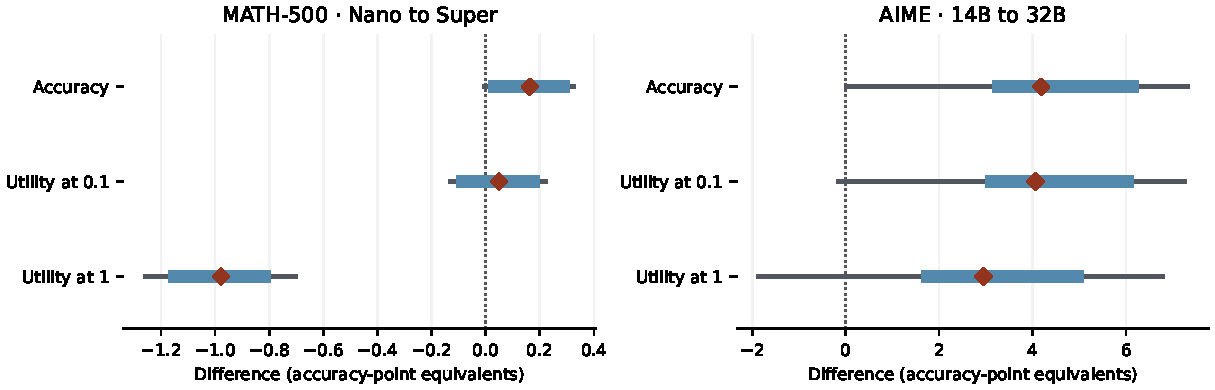
\includegraphics[width=.97\linewidth]{alignment.pdf}
\caption{The length gate minus the call-matched random gate. Thin lines mark question-specific extrema, thick segments mark common extrema, and diamonds mark product pairing. Utility penalties are accuracy points per thousand extra fallback output tokens. The panels use different horizontal scales.}\label{fig:align}
\end{figure}

\paragraph{A pre-answer random comparator can skip work.}
A random router can bypass the first model on requests it escalates. A streaming gate can discard its first response when it observes token $T+1$. With immediate cancellation its first-stage output cost is $\min(L,T+1)$, against $(1-r)L$ in expectation for random bypass. Add this identified first-stage difference to $\rho$ times the aligned fallback-token difference, where $\rho$ is the fallback price relative to the first-stage price per output token. On Nano to Super, the gate saved 183 first-stage tokens per request but still consumed at least 841 additional price-weighted tokens at $\rho=1$. In the Llama comparison the entire cost interval changed sign between $\rho=1$ and $4$, despite an accuracy loss under both. These are counterfactual output-accounting examples conditional on immediate cancellation and full access to emitted tokens.

\begin{table}[htbp]\centering\footnotesize
\caption{Streaming length gate versus pre-answer random bypass. All columns are per incoming request. The fallback point uses the product pairing. Ranges permit question-specific reindexing. The last two columns are weighted token differences in first-stage equivalents. Missing 1.5B telemetry precludes this comparison.}\label{tab:cost}
\begin{tabular}{lrrrrr}
\toprule
Configuration & $\Delta$ first & $\Delta$ fallback & Fallback range & $\rho=1$ & $\rho=4$ \\
\midrule
Nano to Super & -183 & 1142 & [1024, 1255] & [841, 1072] & [3914, 4838] \\
Nano to Llama & -183 & 102 & [78, 131] & [-105, -53] & [129, 339] \\
14B to 32B & 1442 & 1237 & [405, 2109] & [1846, 3551] & [3060, 9878] \\
\bottomrule
\end{tabular}

\end{table}

\paragraph{Independent archive and data audit.}
On the AIME 14B-to-32B pair, all 24 common column permutations favored the recorded-length gate in accuracy. It gained 4.188 points under independent pairing. Even the worst question-specific match retained a small positive margin of 0.022 points. Only two rematched questions could erase its identity-match utility advantage at the one-point penalty. Large favorable accuracy estimates alone give little information about the stability of a cost-sensitive decision.

For the 1.5B first stage, 45 of 120 records had zero recorded output tokens despite containing nonempty answer text, including 11 archived correct responses. Treating the recorded number as the signal is a reproducible audit of that field, but it invalidates a literal interpretation as elapsed generation length. We retain the original analysis in the tables for traceability. We excluded this pair from the streaming cost comparison and repeated both AIME gates using the observed number of Unicode code points in each released answer. We retained the original calibration and test questions, fallback costs and labels. This sensitivity was designed after finding the telemetry problem.
For 1.5B, the character gate escalated 20.8\% of requests at a cutoff of 94,336 characters. Its product accuracy gain was 3.04 points and its common range was $[0.69,4.86]$; the question-specific range $[-1.39,7.99]$ admitted a loss. With 14B first, the cutoff was 1,679 characters, the call rate 24.0\%, and the product gain only 0.89 points. Six of the 24 common permutations favored random escalation, whereas all 24 had favored the token gate. Its question-specific range was $[-3.54,5.84]$. This is a reversal under a simple global change of index convention. Released answer-text length and recorded generation-token usage are different observable signals; the released fields do not establish which generated tokens were displayed. Neither signal can be universally substituted for the other.


\begin{table}[htbp]\centering\footnotesize
\caption{Product accuracy comparisons in points. Keep, Median and Always are alternative fallback rules. Within and Between decompose the primary contrast. The last column repeats that contrast using all questions with the same previously fitted cutoff.}\label{tab:controls}
\begin{tabular}{lrrrrrr}
\toprule
Configuration & Keep & Median & Always & Within & Between & All questions \\
\midrule
Nano to Super & 0.11 & 0.34 & 0.32 & 0.03 & 0.14 & 0.21 \\
Nano to Llama & -13.66 & 5.14 & 7.09 & 0.03 & -8.55 & -7.86 \\
1.5B to 32B & 20.57 & -11.20 & -21.09 & 0.52 & 4.43 & 4.33 \\
14B to 32B & 6.25 & -1.56 & -4.17 & 3.39 & 0.80 & 5.66 \\
\bottomrule
\end{tabular}

\end{table}

\section{Interpretation and limits}
A model-wide reindexing is a sensitivity check for changing a single run-label convention. A question-specific reindexing admits heterogeneous dependence. Neither describes a measured property of an inference service. If both generators are freshly and independently sampled, the product replay is the relevant empirical point. Draw position is a real example of a shared indexing convention even when seeds are model specific. If paired seeds, load conditions or session metadata define the deployment, those conditions should be retained and the permitted mappings restricted accordingly. Very wide arbitrary-coupling ranges can coexist with little variation among uniform shuffles, because an extremal alignment actively selects which fallback answers will count.

The experiments hold the question list, correctness parser, draw pool, gate and model version fixed. A wrong archived grade changes the underlying input. Four AIME draws give only coarse empirical distributions, and changing providers or decoding rules can change all model marginals. The high cutoff is fitted on disjoint questions, but every observed effect remains descriptive of a fixed archive. The token measure omits first-stage latency, input billing, hardware utilization and concurrency. No live system was timed. A conversational fallback that sees a first-stage solution requires conditional generation data. Neither archive identifies that distribution.

\paragraph{Reproducibility and declarations.} The release (\href{https://github.com/fightforbelief/p11-cascade-replay}{GitHub repository}) includes projected records, upstream identifiers and checksums, deterministic policy code, extremizing global permutations, formal execution metadata, and exhaustive small-instance checks. Funding: no specific funding. The authors declare no competing interests.
\begingroup\small
\begin{thebibliography}{10}
\setlength{\itemsep}{2pt}
\bibitem{gupta} N. Gupta et al. Language model cascades: Token-level uncertainty and beyond. ICLR, 2024. \href{https://arxiv.org/abs/2404.10136}{arXiv:2404.10136}.
\bibitem{chen1} T.-R. Chen. What does a routing oracle measure under stochastic decoding? Coupling, scorer choice, and single-commit ceilings. 2026, version 3. \href{https://arxiv.org/abs/2607.03436v3}{arXiv:2607.03436v3}.
\bibitem{chen2} T.-R. Chen. When strong reasoners join the pool: Small union premiums and costly runaway generations in LLM routing. 2026. \href{https://arxiv.org/abs/2611.04098}{arXiv:2611.04098}.
\bibitem{shihab} I. F. Shihab, A. S.-A. M. M. Al Ahsan and M. N. Swaqeeb. Opportunity is not realizability: Selection-valid diagnostics for multi-LLM routing. 2026. \href{https://arxiv.org/abs/2608.08265}{arXiv:2608.08265}.
\bibitem{kuhn} H. W. Kuhn. The Hungarian method for the assignment problem. Naval Research Logistics Quarterly 2, 83--97 (1955). \href{https://doi.org/10.1002/nav.3800020109}{doi:10.1002/nav.3800020109}.
\bibitem{hoeffding} W. Hoeffding. A combinatorial central limit theorem. Annals of Mathematical Statistics 22, 558--566 (1951).
\bibitem{matharena} M. Balunovi\'c, J. Dekoninck, I. Petrov, N. Jovanovi\'c and M. Vechev. MathArena: Evaluating LLMs on uncontaminated math competitions. NeurIPS, 2025. \href{https://doi.org/10.52202/085713-0679}{doi:10.52202/085713-0679}.
\bibitem{data1} T.-R. Chen. Run record and code (NVIDIA B300, MATH-500). \href{https://doi.org/10.5281/zenodo.23939046}{Zenodo, version 23939046}.
\bibitem{data2} MathArena. \href{https://huggingface.co/datasets/MathArena/aime_2025_outputs/tree/16e93d3bb9b0a25ea9422893464d46b3c5ff0ae9}{AIME 2025 outputs}, revision 16e93d3.
\end{thebibliography}
\endgroup
\end{document}
